\documentclass[a4paper]{article}
\usepackage[spanish]{babel}
\usepackage[utf8]{inputenc}
\usepackage{fancyhdr}
\usepackage{charter}   % tipografía
\usepackage{graphicx}
\usepackage{makeidx}

\usepackage{float}
\usepackage{amsmath, amsthm, amssymb}
\usepackage{amsfonts}
\usepackage{sectsty}
\usepackage{wrapfig}
\usepackage{listings} % necesario para el resaltado de sintaxis
\usepackage{caption}
\usepackage{placeins}
\usepackage{longtable}
\usepackage{ulem}

\usepackage{hyperref} % agrega hipervínculos en cada entrada del índice
\hypersetup{          % (en el pdf)
    colorlinks=true,
    linktoc=all,
    citecolor=black,
    filecolor=black,
    linkcolor=black,
    urlcolor=black
}

\usepackage{color} % para snippets de código coloreados
\usepackage{fancybox}  % para el sbox de los snippets de código

\definecolor{litegrey}{gray}{0.94}

% \newenvironment{sidebar}{%
% 	\begin{Sbox}\begin{minipage}{.85\textwidth}}%
% 	{\end{minipage}\end{Sbox}%
% 		\begin{center}\setlength{\fboxsep}{6pt}%
% 		\shadowbox{\TheSbox}\end{center}}
% \newenvironment{warning}{%
% 	\begin{Sbox}\begin{minipage}{.85\textwidth}\sffamily\lite\small\RaggedRight}%
% 	{\end{minipage}\end{Sbox}%
% 		\begin{center}\setlength{\fboxsep}{6pt}%
% 		\colorbox{litegrey}{\TheSbox}\end{center}}

\newenvironment{codesnippet}{%
	\begin{Sbox}\begin{minipage}{\textwidth}\sffamily\small}%
	{\end{minipage}\end{Sbox}%
		\begin{center}%
		\colorbox{litegrey}{\TheSbox}\end{center}}



\usepackage{fancyhdr}
\pagestyle{fancy}

%\renewcommand{\chaptermark}[1]{\markboth{#1}{}}
\renewcommand{\sectionmark}[1]{\markright{\thesection\ - #1}}

\fancyhf{}

\fancyhead[LO]{Sección \rightmark} % \thesection\
\fancyfoot[LO]{\small{Cravero, Mignanelli, Suárez}}
\fancyfoot[RO]{\thepage}
\renewcommand{\headrulewidth}{0.5pt}
\renewcommand{\footrulewidth}{0.5pt}
\setlength{\hoffset}{-0.8in}
\setlength{\textwidth}{16cm}
%\setlength{\hoffset}{-1.1cm}
%\setlength{\textwidth}{16cm}
\setlength{\headsep}{0.5cm}
\setlength{\textheight}{25cm}
\setlength{\voffset}{-0.7in}
\setlength{\headwidth}{\textwidth}
\setlength{\headheight}{13.1pt}

\renewcommand{\baselinestretch}{1.1}  % line spacing


\usepackage{underscore}
\usepackage{caratula}
\usepackage{url}
\usepackage{color}
\usepackage{clrscode3e} % necesario para el pseudocodigo (estilo Cormen)




\begin{document}
%
%\lstset{
%  language=C++,                    % (cambiar al lenguaje correspondiente)
%  backgroundcolor=\color{white},   % choose the background color
%  basicstyle=\footnotesize,        % size of fonts used for the code
%  breaklines=true,                 % automatic line breaking only at whitespace
%  captionpos=b,                    % sets the caption-position to bottom
%  commentstyle=\color{red},    % comment style
%  escapeinside={\%*}{*)},          % if you want to add LaTeX within your code
%  keywordstyle=\color{blue},       % keyword style
%  stringstyle=\color{blue},     % string literal style
%}

\thispagestyle{empty}
\materia{Bases de Datos}
\submateria{Primer Cuatrimestre 2017}
\titulo{Sistema de Inscripción Mundial de Irlanda 2017 (TP1)}
\subtitulo{Taekwon Do World Championship 2017}
\integrante{Lizana, Helen}{118/08}{hsle.22@gmail.com.ar} % por cada integrante (apellido, nombre) (n° libreta) (e-mail)
\integrante{Mignanelli, Alejandro Rubén}{609/11}{minga_titere@hotmail.com} 
\integrante{Sabarros, Ian}{661/11}{iansden@live.com}
\integrante{Sueiro, Diego}{75/90}{dsueiro@gmail.com} 


\maketitle
\newpage

\thispagestyle{empty}
\vfill
%\begin{abstract}
%    \vspace{0.5cm}
%	
%
%\end{abstract}

\thispagestyle{empty}
\vspace{1.5cm}
\tableofcontents
\newpage

%\normalsize
 
\newpage

\section{Introducción}
En el presente trabajo se tratará de proveer un sistema de inscripciones para el Taekwon Do World Championship 2017, teniendo como finalildad, poder aprender a realizar una base de datos en base a un problema del mundo real. Para esto, primero se crearán un Modelo de Entidad Relación y un Modelo Relacional basadas en la especifiación que se encuentra en el enunciado, los cuales usaremos para la creación de una base de datos. Una vez creada, se implementarán las siguientes funcionalidades:

\begin{itemize}
	\item El listado de inscriptos en cada categoría para el armado de llaves
	\item El país que obtuvo mayor cantidad de medallas de oro, plata y bronce.
	\item Sabiendo que las medallas de oro suman 3 puntos, las de plata 2 y las de bronce 1
punto, se quiere realizar un ranking de puntaje por país y otro por escuela.
	\item Dado un competidor, la lista de categorías donde haya participado y el resultado
obtenido.
	\item El medallero por escuela.
	\item El listado de los árbitros por país.
	\item La lista de todos los árbitros que actuaron como árbitro central en las modalidades
de combate
	\item La lista de equipos por país.
\end{itemize}

Para la resolución del problema, hemos decidido utilizar mySql.

\newpage

\section{Aclaraciones}

En esta secci\'on detallaremos características asumidas y que no estan dichas en el enunciado , y aclaraciones sobre la solución:

Asumimos que:

\begin{itemize}

\item Si bien se partía de un modelo más amplio, para los fines de este trabajo solo se modelarán aquellas entidades que cumplen un rol dentro del mismo. Por ello, entidades como Coach o Equipo no fueron modeladas en esta solución.

\end{itemize}

Aclaraciones:

\begin{itemize}

\item En competidores, el campo medalleroPorModalidad contiene una lista con id de modalidades. Cada ves que un competidor gane una medalla en una modalidad, el id de modalidad se agregará a esa lista, aún si ya se encontraba en la misma. medalleroPorCampeonato sigue la misma lógica.

\end{itemize}



\newpage

\section{Desarrollo}

Cuando empezamos a diseñar el DER nos encontramos con varias dudas sobre algunas entidades y alguna de las
relaciones entre ellas. Luego de hacer las consultas con nuestro Tutor tuvimos que realizar algunos cambios. A continuaci\'on describiremos los cambios mas  importantes.

\subsection{Entidad Modalidad}


Una de ellas fue la entidad \textbf{Modalidad}, que por enunciado, solo puede ser de 5 valores posibles y dependiendo del tipo de modo, este posee distintos atributos. Lo primero que se nos ocurrio fue tener una entidad Modalidad como entidad padre y luego como entidades hijas (disjuntas) a cada tipo de modalidad(forma, salto, etc).
Pero eso luego nos tra\'ia complicaciones para definir las relaciones entre Competencia y Modalidad, dado que habia que poner muchas restricciones para que el modelo sea consistente con la especificacion. 
Por ejemplo, si tuviesemos que registrar una competencia con una modalidad del tipo "Forma", una de las restricciones hubiese sido: una competencia debe estar relacionada con uno de los tipos de modalidad. Tambien que solo esta relacionado con el Tipo "Forma" y no pude estar relacionado con otro tipo. 
Tambien habia que aclarar que una competencia podria no estar en la modalidad "Forma". \\

Luego al consultarlo con el Tutor decidimos que no tenia tanta relevacia separar esa informacion en tantas entidades, si no que podr\'iamos almacenar toda esa informacion en una sola entidad. Agregando como restricciones que si la entidad era de detenerminado modo, entonces tenia que tener valores no nulos los atributos correspondientes a ese modo. \\

\subsection{Entidad Competencia}


Al principio pensamos esta entidad como una jerarqu\'ia, Competencia como entidad padre y Sigle y Team como entidades hijas. La entidad Single ser\'ia para las competencias entre competidores, y la entidad Team ser\'ia para las competencias entre equipos. Necesitabamos hacer esto para poder diferenciar que competencias eran de modalidad "combate por equipos" dado que tenia atributos caracter\'sticos. Con esto teniamos cubierto esa diferencia pero al observar m\'as en detalle la existencia de las entidad hijas, vimos que estas no tenian atributos caracteriscos con respecto a su identidad padre, y que en definitiva al pasarlas a la base de datos solo guardar\'ian los campos claves de los competidores/equipos y con un Id de competencia relacionado.\\

Para simplificar el modelo lo que hicimos fue eliminar estas entidades hijas y pasamos la relacion "participa" de Competidor a Competendia y lo mismo para equipo. Y agregamos las restricciones de que una competencia esta relacionada a competidores o a equipos, no puede pasar ambas a la vez.

\subsection{Entidad Match}

Dado que el enunciado ped\'ia obtener los ganadores de cada competencia: 1er, 2do y 3er lugar, pensamos en guardar la informaci\'on de los encuentros y obtener de ellos el resultado de los ganadores. La entidad Match guardar\'ia el id del competidor ganador y la fecha del encuentro. Para esto asumiamos que los dos \'ultimos encuentros ser\'ian las del 3er puesto y la final. Aca nos volvimos a encontrar con el problema de diferenciar los encuentros entre competidores y los de equipos, por lo cual teniamos que crear una jerarquia para obtener MatchIndividual y MatchGrupo. Y al igual que en el caso de la entidad Competencia ,estas entidades hijas carecian de atributos y s\'olo guardaban campos claves de otras entidades.

Luego de mostrarselo al Tutor, comprendimos que no habia que guardar la informacion de los encuentros, y que s\'olo
bastaba con que la competencia almacenara los Id de los competidores/equipos ganadores. Por ese decidimos eliminar la entidad Match y agregar los atributos necesarios a la Entidad Competencia para que guarde la informaci\'on de los ganadores.







\newpage

\section{Modelo de Entidad Relación y Modelo Relacional}

A continuación, se mostrarán el Modelo de Entidad Relación y el Modelo Relacional correspondientes a nuestra solución del problema.\\

\subsection{Modelo de Entidad Relación}


\begin{center}
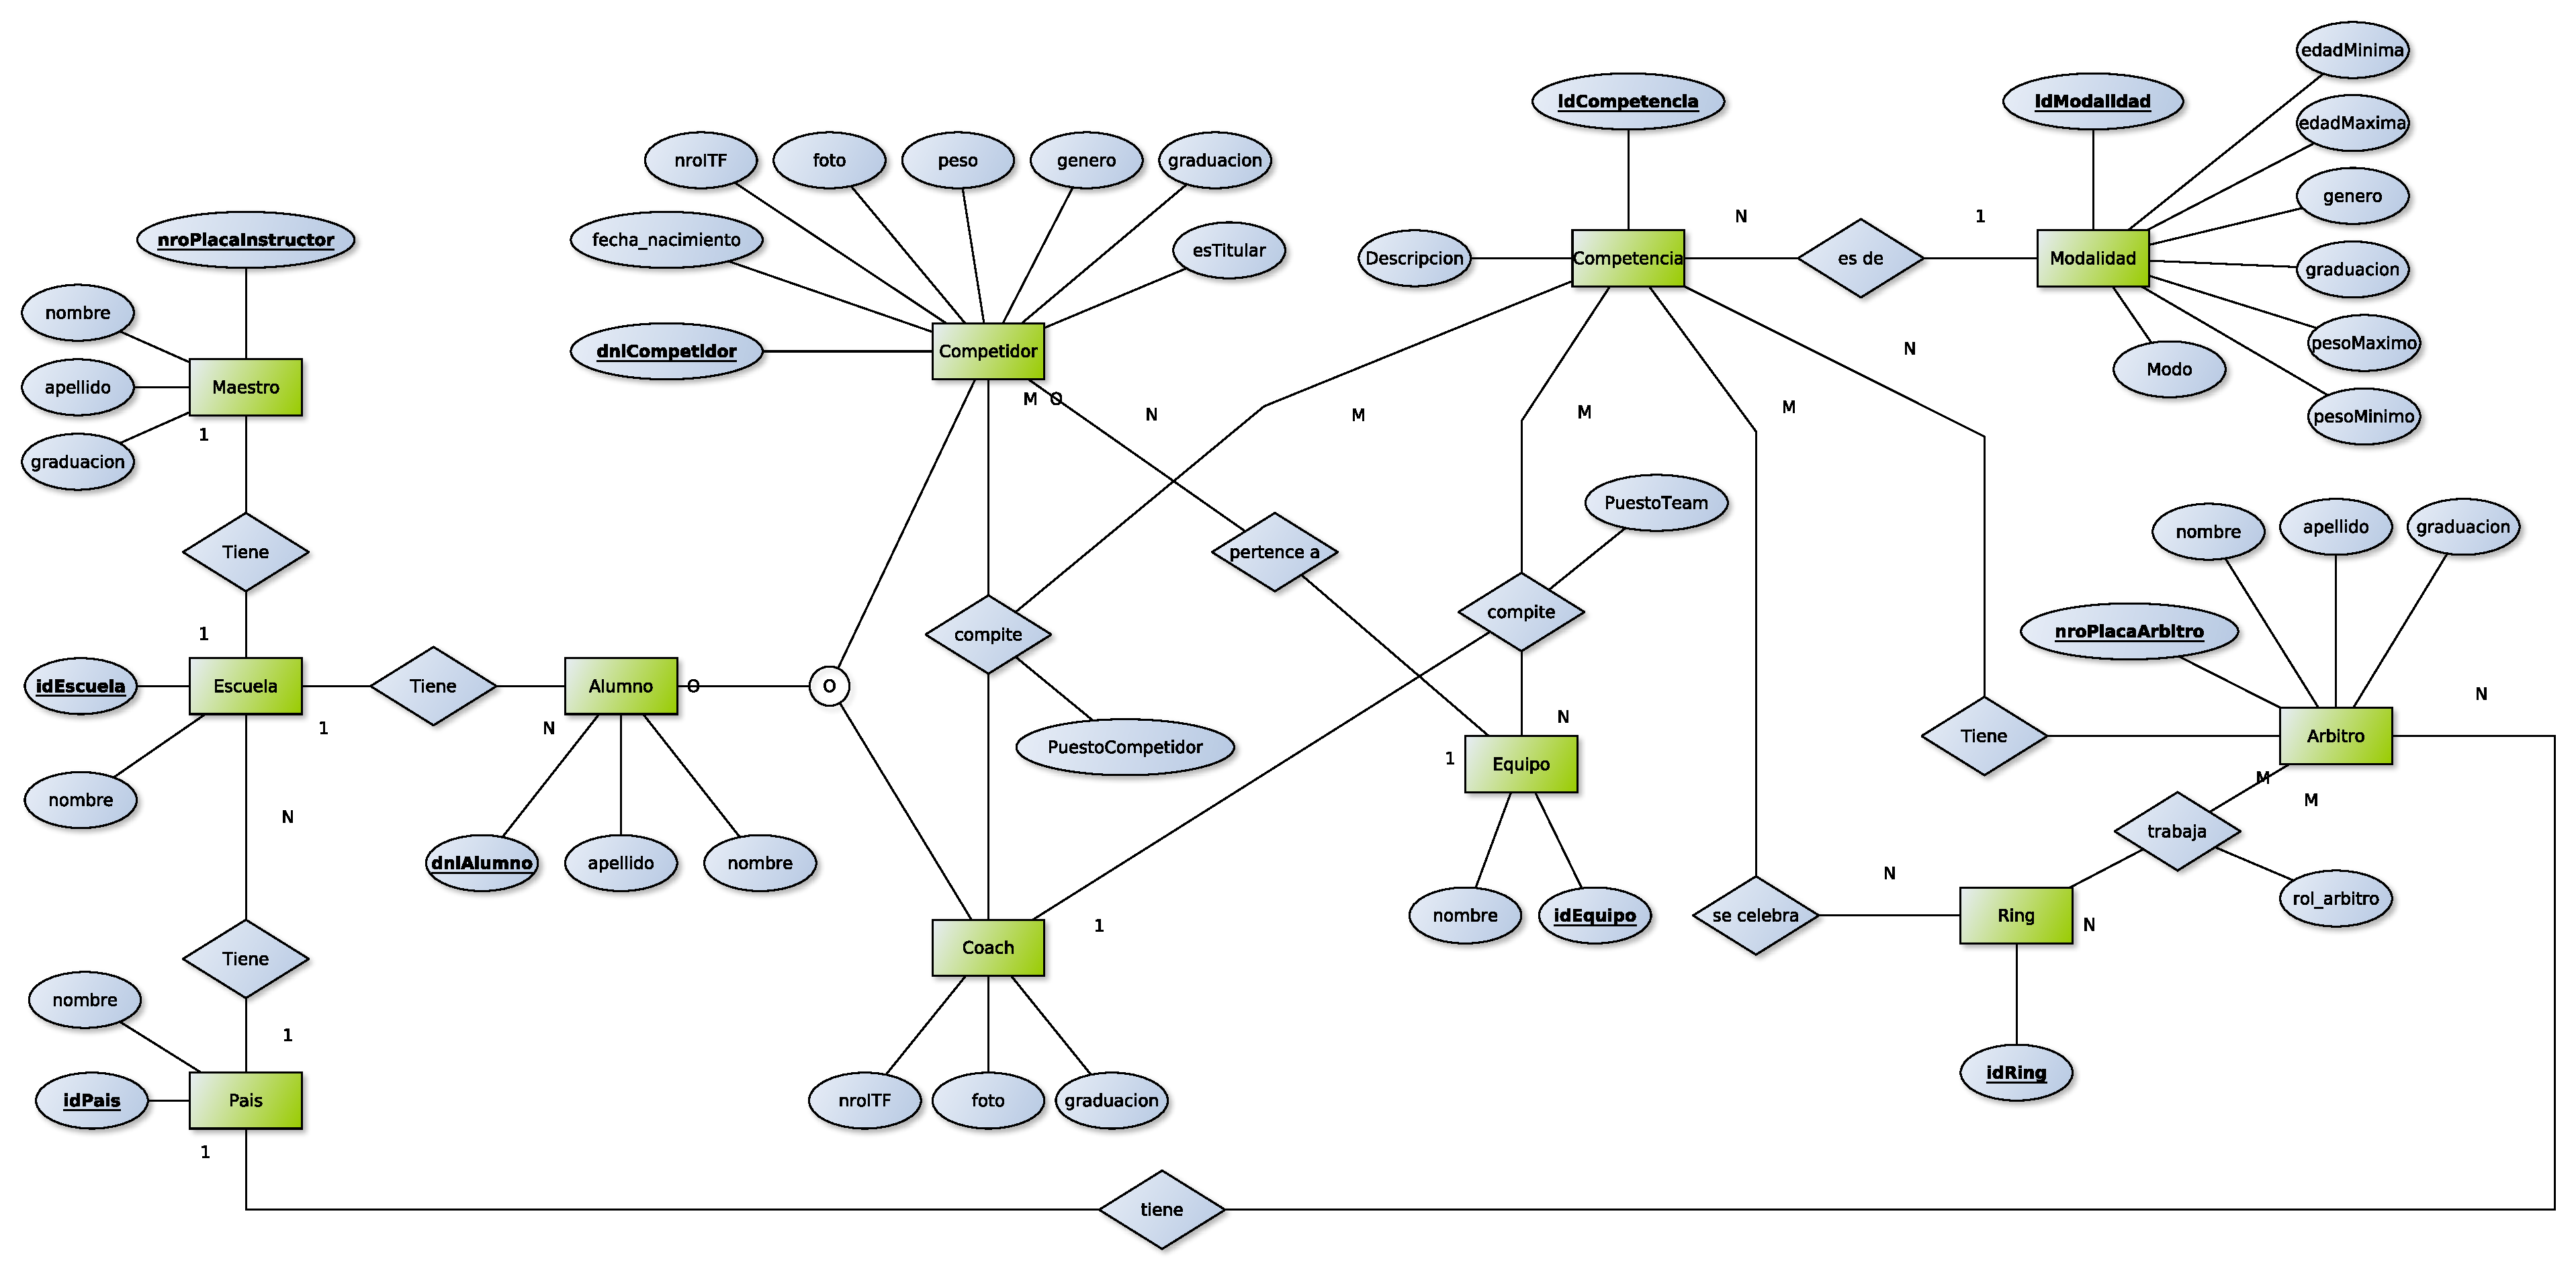
\includegraphics[width=20cm,keepaspectratio,angle=90]{./imagenes/DER.pdf}\newline
\end{center}

\newpage
\subsection{Modelo Relacional}

\noindent\textbf{Escuela}(\uline{idEscuela}, nombre, \dashuline{idPais}, \dashuline{nroPlacaInstructor}) 
\\
\\
PK = CK = \{ idEscuela \} \\
FK = \{ idPais, nroPlacaInstructor \} \\

\begin{verbatim}
--------------------------------------------------------------------------
\end{verbatim}

\noindent\textbf{Pais}(\uline{idPais}, nombre)
\\
\\
PK = CK = \{ idPais \} \\


\begin{verbatim}
--------------------------------------------------------------------------
\end{verbatim}

\noindent\textbf{Maestro}(\uline{nroPlacaInstructor}, nombre, apellido, graduación)
\\
\\
PK = CK = \{ nroPlacaInstructor \} \\


\begin{verbatim}
--------------------------------------------------------------------------
\end{verbatim}

\noindent\textbf{Alumno}(\uline{dniAlumno}, nombre, apellido, \dashuline{idEscuela})
\\
\\
PK = CK = \{ dniAlumno \} \\
FK = \{ idEscuela \} \\

\textit{Restricciones:}
\begin{itemize}
	\item un Alumno puede ser coach y competidor a la vez.
\end{itemize}

\begin{verbatim}
--------------------------------------------------------------------------
\end{verbatim}

\noindent\textbf{Coach}(\uuline{dniAlumno}, nroITF, foto, graduación)
\\
\\
PK = CK = FK = \{ dniAlumno \} \\

\textit{Restricciones:}
\begin{itemize}
	\item Un alumno puede \textbf{no} estar en Coach
	\item habrá al menos un coach por cada 5 competidores
\end{itemize}


\begin{verbatim}
--------------------------------------------------------------------------
\end{verbatim}

\noindent\textbf{Competidor}(\uuline{dniAlumno}, nroITF, fechaNacimiento, género, graduación, peso, foto, esTitular, \dashuline{idEquipo})
\\
\\
PK = CK = \{ dniCompetidor \} \\
FK = \{ idEquipo \} \\


\textit{Restricciones:}
\begin{itemize}
	\item Un alumno puede \textbf{no} estar en Competidor.
	\item El Competidor puede \textbf{no} estar en Equipo.
	\item Si el Competidor está en Equipo, entonces si es titular, el campo esTitular tendrá un True, y si es suplente tendrá un false. En caso de no tener equipo, ese campo contendrá null.
\end{itemize}

\begin{verbatim}
--------------------------------------------------------------------------
\end{verbatim}

\noindent\textbf{Equipo}(\uline{idEquipo}, nombre)
\\
\\
PK = CK = \{ idEquipo \} \\

\textit{Restricciones:}
\begin{itemize}
	\item Los equipos están conformados por 5 titulares y 3 suplentes, y todos deben ser de la misma escuela.
\end{itemize}


\begin{verbatim}
--------------------------------------------------------------------------
\end{verbatim}

\noindent\textbf{Competencia}(\uline{idCompetencia}, descripcion, \dashuline{idModalidad})
\\
\\
PK = CK = \{ idCompetencia \} \\
FK = \{ idModalidad \} \\

\begin{verbatim}
--------------------------------------------------------------------------
\end{verbatim}

\noindent\textbf{compiteEnCompetenciaInd}(\uuline{dniCompetidor}, \uuline{idCompetencia}, \dashuline{dniCoach}, puestoCompetidor)
\\
\\
PK = \{ (dniCompetidor,idCompetencia) \} \\
CK = \{ (dniCompetidor,idCompetencia), (dniCompetidor,dniCoach), (idCompetencia,dniCoach)\} \\
FK = \{ dniCompetidor, idCompetencia, dniCoach \} \\

\textit{Restricciones:}
\begin{itemize}
	\item Los competidores que se registren en una competencia, deben cumplir con las exigencias de la misma, es decir, deben respetar la edad, el sexo, la graduación, o cualquier exigencia que la modalidad de la competencia exija.
	\item Un coach que es competidor no podrá ser coach de si mismo.
\end{itemize}


\begin{verbatim}
--------------------------------------------------------------------------
\end{verbatim}

\noindent\textbf{compiteEnCompetenciaTeam}(\uuline{idEquipo}, \uuline{idCompetencia}, \dashuline{dniCoach}, puestoTeam)
\\
\\
PK = \{ (idEquipo,idCompetencia) \} \\
CK = \{ (idEquipo,idCompetencia), (idEquipo,idCompetencia), (idCompetencia,dniCoach)\} \\
FK = \{ idEquipo, idCompetencia, dniCoach \} \\

\textit{Restricciones:}
\begin{itemize}
	\item Los competidores de los equipos que se registren en una competencia, deben cumplir con las exigencias de la misma, es decir, deben respetar la edad, el sexo, la graduación, o cualquier exigencia que la modalidad de la competencia exija.
	\item Un coach que es competidor no podrá ser coach del equipo al que pertenece.
\end{itemize}

\begin{verbatim}
--------------------------------------------------------------------------
\end{verbatim}

\noindent\textbf{Modalidad}(\uline{idModalidad}, edadMínima, edadMáxima, género, graduación, pesoMínimo, pesoMáximo, modo)
\\
\\
PK = CK = \{ idModalidad \} \\
\textit{Restricciones:}
\begin{itemize}
	\item Los modos determinan que atributos deben estar en null según lo pedido en el enunciado.
\end{itemize}


\begin{verbatim}
--------------------------------------------------------------------------
\end{verbatim}

\noindent\textbf{Ring}(\uline{idRing})
\\
\\
PK = CK = \{ idRing \} \\

\begin{verbatim}
--------------------------------------------------------------------------
\end{verbatim}

\noindent\textbf{Arbitro}(\uline{nroPlacaArbitro}, nombre, apellido, graduación, \dashuline{idPais})
\\
\\
PK = CK = \{ nroPlacaArbitro \} \\
FK = \{ idPais \} \\

\begin{verbatim}
--------------------------------------------------------------------------
\end{verbatim}

\noindent\textbf{arbitrosEnCompetencias}(\uuline{nroPlacaArbitro}, \uuline{idCompetencia})
\\
\\
PK = CK = FK = \{ (nroPlacaArbitro,idCompetencia) \} \\

\textit{Restricciones:}
\begin{itemize}
	\item La graduación de un arbitro debe ser siempre MAYOR a la graduación de la modalidad de la competencia.
\end{itemize}

\begin{verbatim}
--------------------------------------------------------------------------
\end{verbatim}

\noindent\textbf{ringsDeCompetencias}(\uuline{idRing}, \uuline{idCompetencia})
\\
\\
PK = CK = FK = \{ (idRing,idCompetencia) \} \\

\textit{Restricciones:}
\begin{itemize}
	\item Los rings de cada competencia deben poseer arbitros que tengan la capacidad de dirigirlas.
\end{itemize}

\begin{verbatim}
--------------------------------------------------------------------------
\end{verbatim}

\noindent\textbf{puestoArbitroEnRing}(\uuline{nroPlacaArbitro},\uuline{idRing}, puesto)
\\
\\
PK = CK = FK = \{ (nroPlacaArbitro,idRing) \} \\

\textit{Restricciones:}
\begin{itemize}
	\item En un Ring siempre habrá un presidente de mesa, un arbitro central, varios jueces y al menos tres suplentes.
\end{itemize}

\begin{verbatim}
--------------------------------------------------------------------------
\end{verbatim}

\newpage

\section{Entorno y Código}

La base ha sido desarrollada en mySql y se encuentra bajo el nombre taekwondo.sql en la carpeta SQL que se adjunta junto con el informe. Las querys están en la misma carpeta numeradas desde Ejercicio1.sql hasta Ejercicio8.sql . 

\section{Conclusiones}

A lo largo del trabajo, nos encontramos con muchas cuestiones de decisión, en la clásica lucha claridad VS mantenimiento. Originalmente teníamos aproximadamente 24 entidades, que fueron recortadas a un total de 11, puesto que mantener la consistencia de tantas tablas resultaba mucho más costoso en nuestra opinión, que la perdida de claridad al tener menos entidades que almacenaran la misma información. Por otro lado, pudimos apreciar de primera mano como el pasaje del DER al MR y del MR a la base no es tan directo como la teoría podría sugerir, puesto que al realizar la base, nos hemos encontrado que cierta información resultaban muy complicadas de ser accedidas mediante querys por la estructura de la base, lo cual termino provocando en cambios en esta, que luego escalaron a cambios en el MR y obviamente en el DER. Finalizando, también experimentamos la complejidad de armar la estructura de una base en un conjunto de 4 personas, puesto que la diferencia de opiniones sobre un mismo enunciado, impacto gravemente en la definición de entidades, lo cual repercute eventualmente en la generación de la base.

En conclusión, consideramos que se alcanzaron los objetivos propuestos en este trabajo, puesto que pudimos toparnos y resolver de una manera que consideramos correcta, un ejemplo de la vida real sobre bases de datos.

\end{document}

